\section{Resultados}

A implimentação utilizando ThreadPools foi dedcidida pois é a mais fácil de encontrar bugs, pois a cada iteração de disparo é feito a sincronização e a escrita em dados. Houve várias tentativas de manter totalmente em paralelo, mas ão consegui encontrar problemas de sincronia em escrita de arquivos.

Além do \textit{tradeoff} do atraso do trabalho teve o problema do gargalo. Por exemplo nas figuras \ref{fig3} e \ref{fig4}.

\begin{figure}
  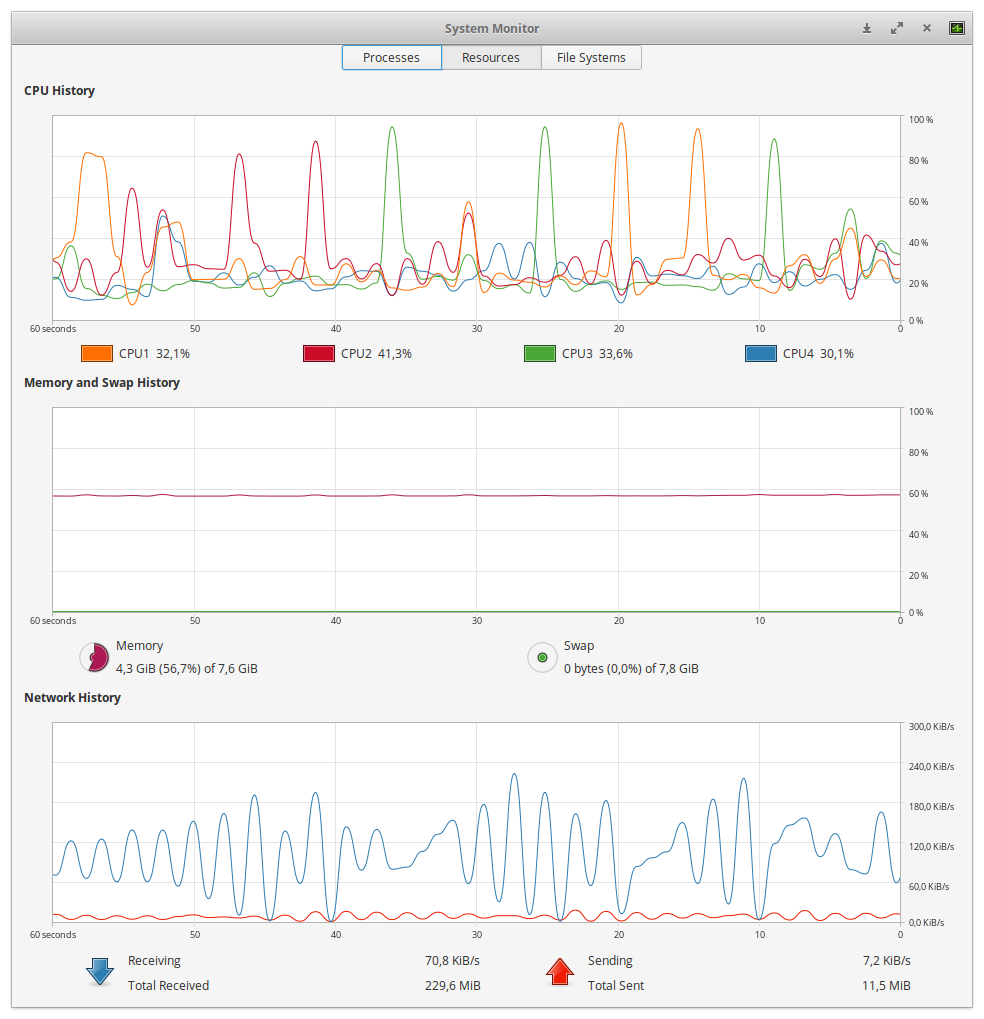
\includegraphics[width=0.5\textwidth]{images/monitor.png}
  \caption{Uso de CPU, RAM e Rede no início}
  \label{fig3}
\end{figure}

Em que após algumas iterações ocorrem atrasos que não foram possíveis serem sanados.

Os possíveis erros são:

\begin{itemize}
  \item complexidade de links colectados no Spider
  \item má utilização da classe vector do cpp
  \begin{itemize}
    \item muitos \textbf{inserts} e \textbf{erase} utilizados
  \end{itemize}
\end{itemize}

\begin{figure}
  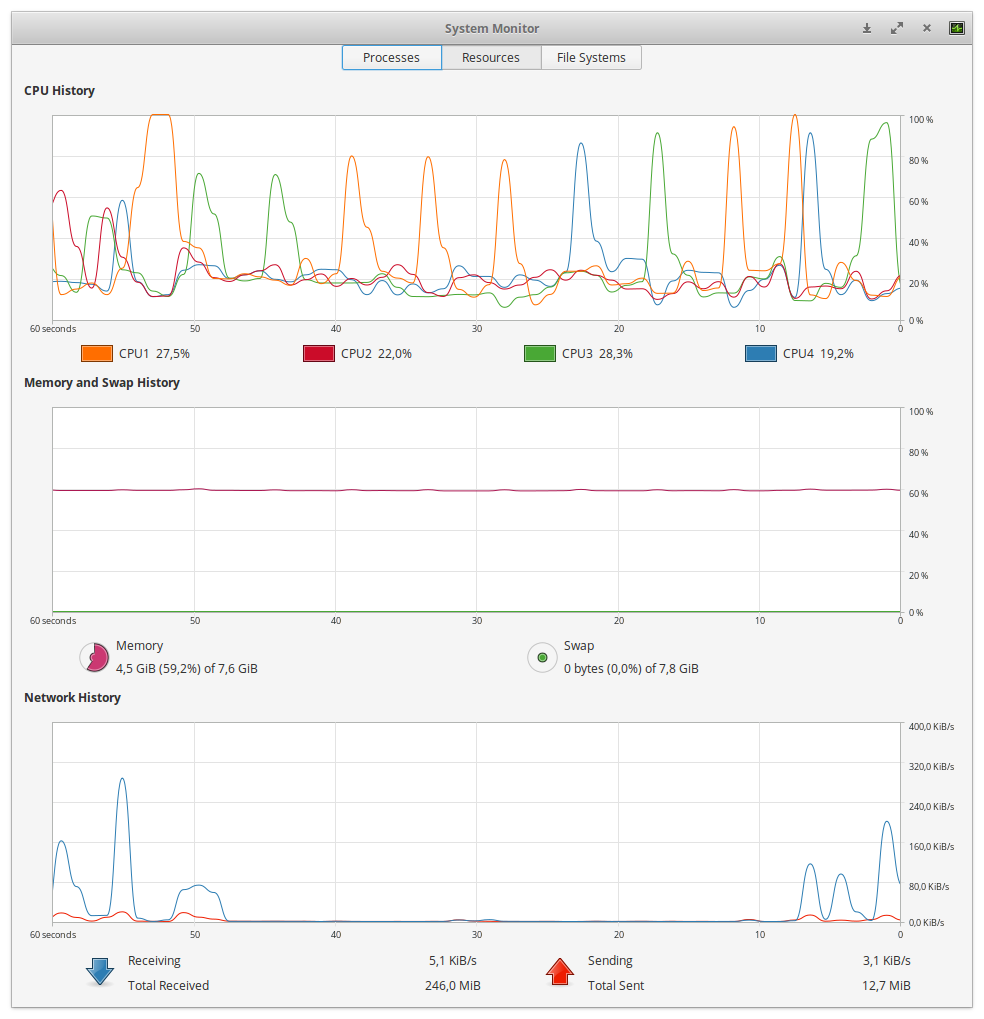
\includegraphics[width=0.5\textwidth]{images/monitorwithgargalo.png}
  \caption{Uso de CPU, RAM e Rede com gargalo}
  \label{fig4}
\end{figure}

\subsection{Coleção}

A quantidade de páginas coletadas foram \textbf{27114} páginas, através dos UniqueIDs criados, e o dump da coleção foi de \textbf{2,9GB}. Que considerado bem pouco, mas foi ocasionado pelo uso de detecção de UniqueIDs e ciclos no grafo da Web que eu não consegui sanar (afinal, era desejado baixar sites que são atualizados depois de um tempo).

O crescimento da coleção se tornou logarítmica, pois depois de uma hora já continha 1GB, mas no final do dia foi coletado no total de 2GB.

\begin{figure}[h]
  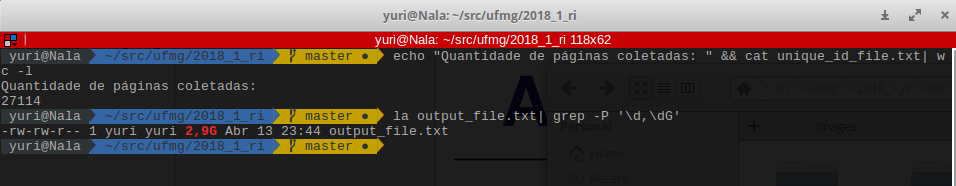
\includegraphics[width=0.5\textwidth]{images/sizecollected.png}
  \caption{Quantidade de páginas coletadas}
  \label{}
\end{figure}
